\documentclass[tikz,border=3pt]{standalone}
\usepackage[utf8]{inputenc}
\usepackage[T1]{fontenc}
\usepackage{lmodern}
\renewcommand{\familydefault}{\sfdefault}
\usepackage{sansmath}\sansmath
\usepackage{chemfig}
\usepackage{pgfplots}\pgfplotsset{compat=1.18,/pgf/number format/use comma,/pgf/number format/1000 sep={.}}
\usetikzlibrary{arrows.meta,calc,positioning,decorations.pathmorphing,patterns}
% paleta del sitio
\definecolor{nar}{HTML}{E8680C}\definecolor{narc}{HTML}{FFB35C}\definecolor{hielo}{HTML}{FFF3E8}
\definecolor{tinta}{HTML}{1D1D1F}\definecolor{gris}{HTML}{6E6E73}\definecolor{lila}{HTML}{7C5CF0}
\definecolor{azul}{HTML}{2F6FD6}\definecolor{menta}{HTML}{17A673}\definecolor{coral}{HTML}{E8342A}
\begin{document}
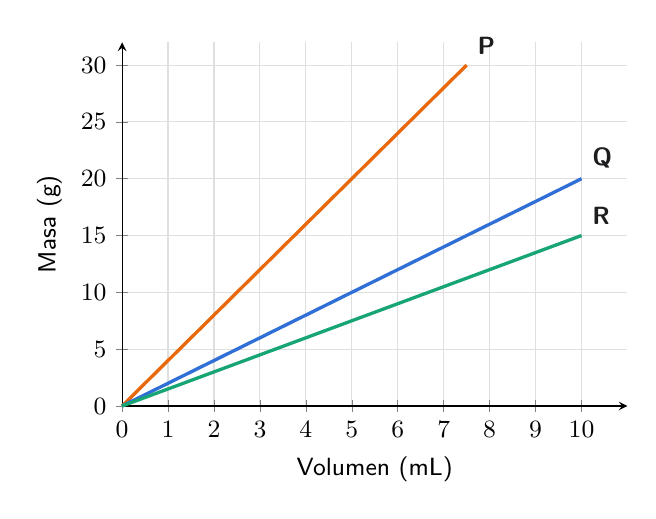
\begin{tikzpicture}[font=\small]
\begin{axis}[axis lines=left,grid=major,grid style={gray!25},xlabel={Volumen (mL)},ylabel={Masa (g)},width=8cm,height=6.2cm,xmin=0,xmax=11,ymin=0,ymax=32,xtick={0,1,...,10},ytick={0,5,...,30},clip=false]
\addplot[nar,very thick] coordinates {(0,0)(7.5,30)} node[anchor=south west,font=\small\bfseries,text=tinta] {P};
\addplot[azul,very thick] coordinates {(0,0)(10,20)} node[anchor=south west,font=\small\bfseries,text=tinta] {Q};
\addplot[menta,very thick] coordinates {(0,0)(10,15)} node[anchor=south west,font=\small\bfseries,text=tinta] {R};

\end{axis}
\end{tikzpicture}
\end{document}
